\documentclass[12pt]{article}
\usepackage[utf8]{inputenc}
\usepackage[margin=3em]{geometry}
\usepackage{tabularx}
\usepackage{graphicx}
\usepackage{xcolor}
\usepackage{lmodern}
\usepackage{listings}
\lstset{language=,
    basicstyle=\sffamily\footnotesize,
    xleftmargin=20pt,
    xrightmargin=20pt,
    numbers=left,
    stepnumber=1, % le pas des numeros de ligne
    numbersep=10pt,
    breaklines=true,
    tabsize=4,
    %frame=single,
    showspaces=false,
    showstringspaces=false
    inputencoding=utf8, %put1 d'utf8 dans listing
    extendedchars=true, %put1 d'utf8 dans listing
    columns=fullflexible, % suppression des espaces autour des deux-points
    escapechar=`, % permet d'insérer du §code latex§
    backgroundcolor=\color{lightgray},
    keywordstyle=\hlc,
    morecomment=[l]{\#}, % commentaires shell en ligne
    commentstyle=\itshape\color{darkgray},
}



\begin{document}

\title{MAP:\\Developer guide}
\maketitle

\tableofcontents
\newpage

This document purpose is to gives elements to permit everyone to adapt MAP to
their needs or help us extending it.\\
Almost all the solution is written in python. The code itself is then easily
readable/modifiable.\\[1\baselineskip]
\textbf{Note:} When designing MAP, we more tried to give a proof of concept that a ready-to-use solution. This is why devices and ports are identified by their name or hostname instead of real ID, as used in openstack. This should be changed in future versions.

\section{Solution overview}
This section will present MAP goals and architecture.

\subsection{Current openstack approach}
It is not necessary to understand how works openstack to understand MAP or
develop on it. This section is just here to help you if you come from
openstack/neutron's world by highlihting major differences.\\
Currently, neutron is not awared of the physical network. When a VM is
created/deleted/migrated, nova just asks neutron to keep
up-to-date a database
containing all information regarding virtual networks. Nova take care of
creating VM/VNics and plugs VNics on virtal switches. Neutron agent,
discovering new or missing VNics ask neutron plugin that returns rules
concerning new VNics (Vlan or other, segment\_id..).
\begin{figure}
    \begin{center}
        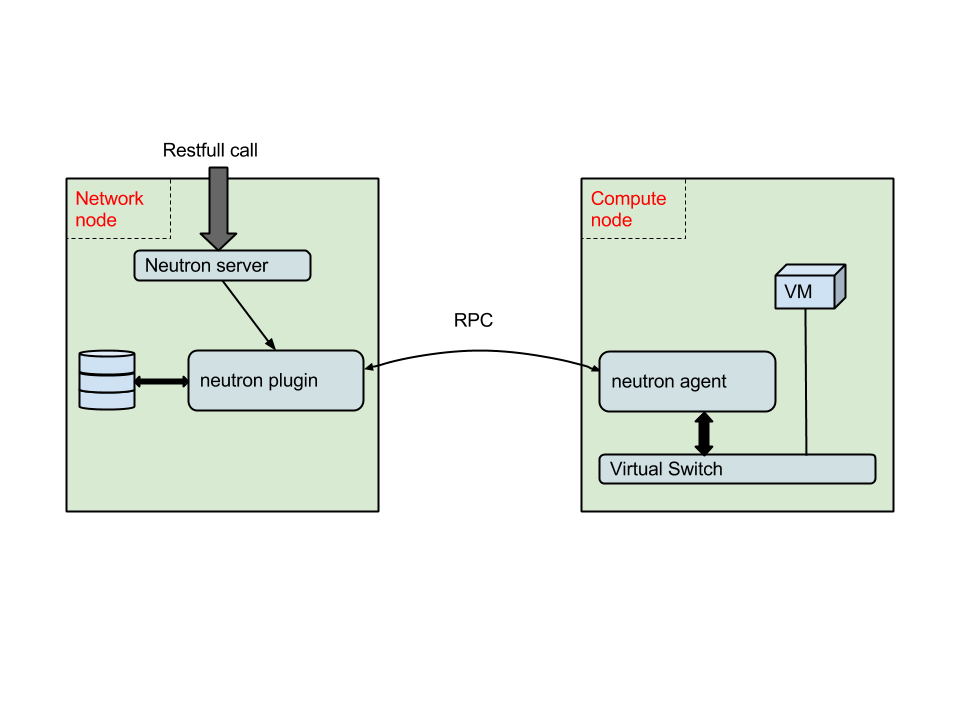
\includegraphics[width=400pt]{img/old_neutron.png}
        \caption{Current neutron architecture}
    \end{center}
\end{figure}
Services to apply are in fact found in the plugin configuration files, where
you specify using vlan or tunnels and vlan/tunnels range that may be used.

\subsection{Global architecture}
Contrary to openstack approach, MAP takes in consideration the whole network. It
keeps a network abstract representation. Over this network, a sort of 'network
controller' runs. This controller receives neutron-server calls (north-bound).
It then chooses isolation methods to set-up on the network (ex: vlan) and ask
some drivers (south-bound) to apply those changes.
\begin{figure}
    \begin{center}
        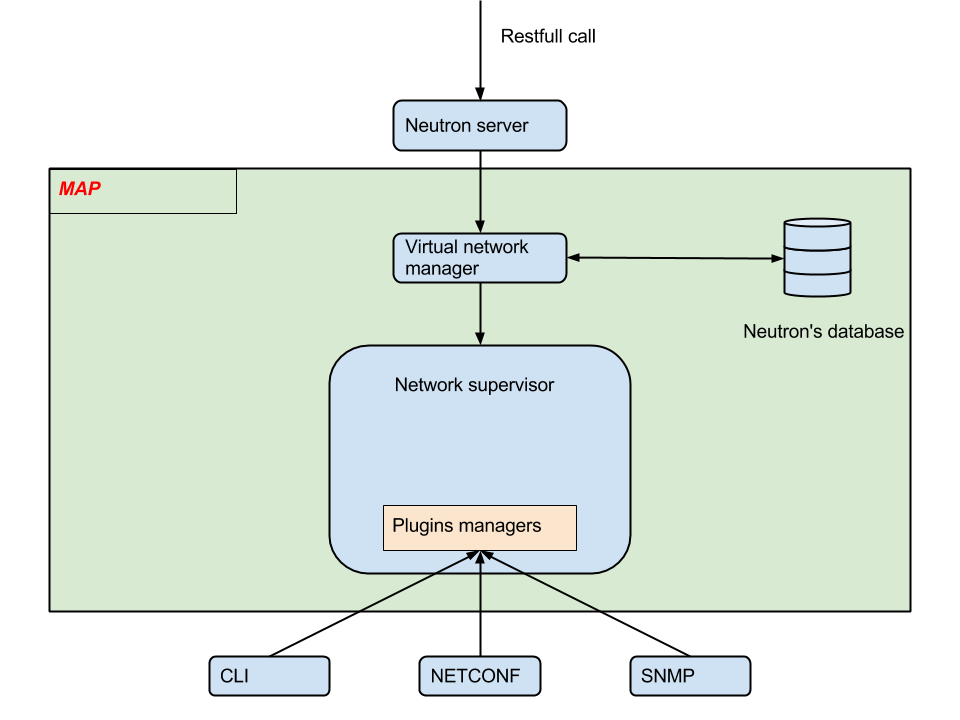
\includegraphics[width=400pt]{img/MAP.png}
        \caption{MAP architecture}
    \end{center}
\end{figure}
Controller itself is a bunch of modules. Each module is in charge for a
determined task.
\begin{figure}
    \begin{center}
        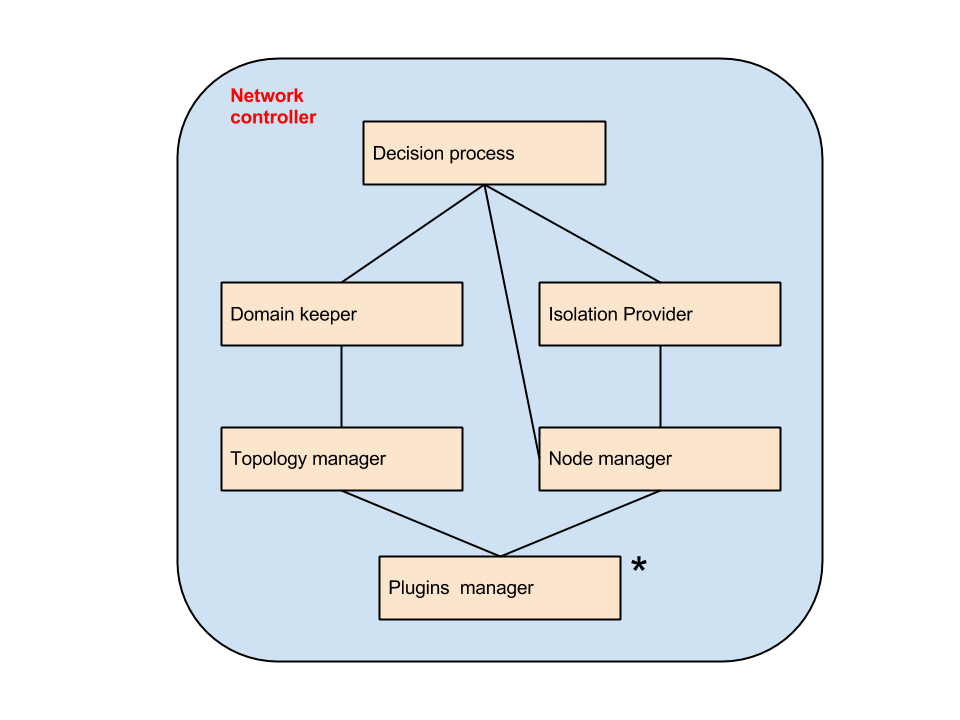
\includegraphics[width=400pt]{img/controller.png}
        \caption{Controller modules and their interraction}
    \end{center}
\end{figure}

\section{Modules}
\subsection{Node manager}
\subsubsection{Role}
A network is basically a set of nodes and link. Node manager keeps an abstract
representation of nodes under the form of MetaCLI (XML) files containing devices
configurations. A more accurate representation would probably have contained the
exact state of the device (including up/down ports, services...). This
representation only uses configuration however.\\
Most of node manager's work is achieved thanks to PyXB, an xml library ensuring respect of XML 
schemas.\\
Node manager (and every other modules) does \textbf{not} acces files directly.
A special class, \emph{ManagerDb}, in file \emph{\textbf{ressources.py}} is used as
an interface between files and PyXB objects.\\
\subsubsection{API}
Node manager gives an API to work on devices configurations~:\\[1\baselineskip]

\textbf{deploy\_service(self, device\_name, instance\_service\_name):}
\begin{description}
    \item[in:] \hfill \\
        \begin{itemize}
            \item device\_name: name of the concerned device
            \item instance\_service\_name : an instance specific to a device and its interfaces(ports).
        \end{itemize}
    \item[out:] \hfill \\
        \begin{itemize}
            \item returns None, device XML file is updates
        \end{itemize}
\end{description}
Instance nodes are added to device xml tree by this method. It correspond to a service deployment on a device.\\

Decisions taken by decision process can end up removing services (services instances) from devices. This can be achieved with the following method~:\\[1\baselineskip]

\textbf{remove\_service(self, device\_name, instance\_service\_name):}
\begin{description}
    \item[in:] \hfill \\
        \begin{itemize}
            \item device\_name: name of the concerned device
            \item instance\_service\_name : an instance specific to a device and its interfaces(ports).
        \end{itemize}
    \item[out:] \hfill \\
        \begin{itemize}
            \item returns None, device XML file is updates
        \end{itemize}
\end{description}
When network topology is modified, a notification permits to update this module to take in consideration new devices. Those devices should be manually added with authentication processes. With appropriate driver (currently not implemented), openflow devices may be automatically added. Authentication processes are only handled by devices managers like netconf driver. Node manager only needs to know about device configuration.\\[1\baselineskip]

\textbf{update\_node(node, state, configuration):}
\begin{description}
    \item[in:] \hfill \\
        \begin{itemize}
            \item node: targeted device ID
            \item state: update type: ADD, DEL
            \item conf: node configuration in device (native) format
        \end{itemize}
\end{description}
Updates node with state ADD or DEL\\

\subsubsection{Files}
Node manager is almost completely contained in file \emph{\textbf{nodemanager.py}}. This file contains required functions to manage services over devices.\\
To achieve its goal, Node manager uses validation rules on deployment. A separate module found in \emph{\textbf{validator.py}} focuses on validation. It is helped by validation operations that can be found in \emph{\textbf{operationvalidation.py}}\\
Devices represented as XML are stored in a \emph{network} directory. This directory is refered in MAP configuration by \emph{network\_path} option.


\subsection{Isolation provider}
\subsubsection{Role}
Isolation provider is a module in charge for knowing and providing different means of separating tenant networks. Vlan is a highly used solution but many others, like GRE, VPN, MPLS or soon OTV, VxLAN, or NVGRE, could be better alternatives.\\
For each isolation method (often network services), Isolation provider keep a 'generic service' file. This file is an XML file conforming to MetaCLI syntax. Generic service sum-up all parameters that should be set in a device configuration to deploy this service. Decision process will interact with Isolation provider to get a 'service instance' ready to be deployed on devices. A service instance matches a generic service but contains parameters set with appropriate values. It can then be applied on XML devices configurations.

\subsubsection{API}
\textbf{list\_services\_by\_devices(method, devices):}
\begin{description}
    \item[in:] \hfill \\
        \begin{itemize}
            \item method: list of method
            \item devices: list of devices
        \end{itemize}
    \item[out:] \hfill \\
        \begin{itemize}
            \item list of method extracted from given method list containing methods supported by all given devices
        \end{itemize}
\end{description}

\textbf{list\_services\_by\_domain(domain):}
\begin{description}
    \item[in:] \hfill \\
        \begin{itemize}
            \item domain: domain type (ex: ‘l2’ or ‘l3’)
        \end{itemize}
    \item[out:] \hfill \\
        \begin{itemize}
            \item list of services names
        \end{itemize}
\end{description}
Isolation provider creates isolation instances from generic isolation methods, each instance depends on : Device\_name, interface\_name, service\_id, and all devices in relation with this service instance~:\\[1\baselineskip]
\textbf{create\_service\_instance(self, service\_name, service\_id, devices\_ports):}
\begin{description}
    \item[in:] \hfill \\
        \begin{itemize}
            \item service\_name: ex: vlan, trunk ...
            \item service\_id: ex: vlan number for vlan service
            \item devices\_ports: all devices and their ports concerned by this instance
        \end{itemize}
    \item[out:] \hfill \\
        \begin{itemize}
            \item XML files for all instances in ValidMakerDB
        \end{itemize}
\end{description}

\subsubsection{Files}
Isolation provider can be found in \emph{\textbf{isolationprovider.py}}. It does \textbf{not} acces files directly and uses DbManager (\emph{\textbf{ressources.py}}). It works with generic service files, found in directory pointed out by MAP configuration file, option \emph{service\_path}.

\subsection{Topology manager}
\subsubsection{Role}
Topology manager is complementary with Node manager. When abstracting networks by a set of nodes and links, Node manager is concerned by nodes. Topology manager manages links between those nodes. Its main activity is to construct, store and query a port matrix. A port matrix is a set of devices appearing on both rows and columns. A cross between a row and a column contains the port (if there is any) used by row device to access column device.
\begin{figure}
    \begin{center}
        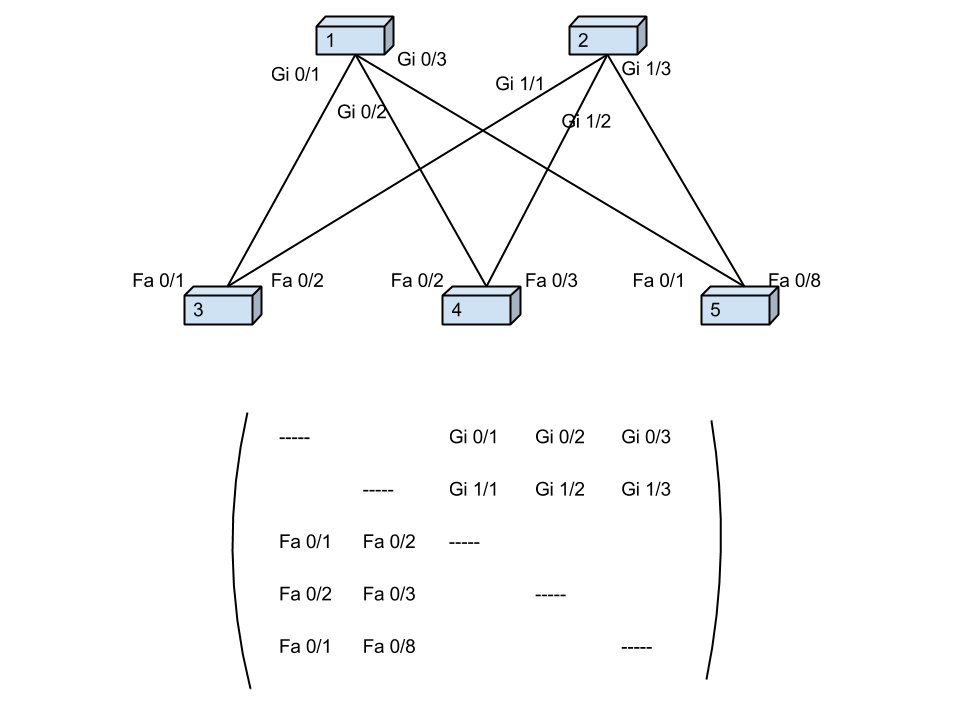
\includegraphics[width=400pt]{img/pmatrix.png}
        \caption{Port matrix example}
    \end{center}
\end{figure}

\subsubsection{API}
\textbf{get\_paths(hosts):}\\
Paths are calculated recursively. When given hosts, Topology manager found all paths between hosts and returns all ports (needing to be configured) by concatenation. Indeed, if two paths exist between host1 and host2, both needs to be configured. If the first path go down, the second will be used. This is why this second path should also be configured for supporting a virtual network between host1 and host2.\\
\begin{description}
    \item[in:] \hfill \\
        \begin{itemize}
            \item hosts: list of host\_id
        \end{itemize}
    \item[out:] \hfill \\
        \begin{itemize}
            \item ordered list of path with devices and ports concerned.
        \end{itemize}
\end{description}
When building MAP, we hoped to bring it to a higher level of automation. Currently, nodes/links must be specified manually. But thanks to many existing protocols, it could be possible to detect many modification on the underlying network. That should be done by adding drivers 'monitoring' the network (ex:SNMP listener), and notifying our plugin of network modifications.
This manager should then receive updates from drivers. Two function can be called, to notify a node or link modification~:\\[1\baselineskip]
\textbf{update\_node(node, state):}\\
Update the node with state ADD or DEL
\begin{description}
    \item[in:] \hfill \\
        \begin{itemize}
            \item node: Node ID to modify
            \item state: Update type. ADD, DEL
        \end{itemize}
\end{description}

\textbf{update\_link(host\_src, port\_src, host\_dest, port\_dest, state):}\\
Update the link with state UP or DOWN
\begin{description}
    \item[in:] \hfill \\
        \begin{itemize}
            \item host\_src: source host’s ID
            \item port\_src: source interface name
            \item host\_dest: destination host’s ID
            \item port\_dest: destination interface name
            \item state: ‘UP’ or ‘DOWN’
        \end{itemize}
\end{description}

We also use a function to add a broadcast space. All devices in this space can exchange packets as if they were directly connected one to another. Broadcast spaces are defined by a set of nodes and an ID.\\[1\baselineskip]
\textbf{add\_broadcast\_space(broadcast\_devices):}\\
Add broadcasting spaces in the database
\begin{description}
    \item[in:] \hfill \\
        \begin{itemize}
            \item broadcast\_devices : nodes to add in a new broadcast domain
        \end{itemize}
\end{description}

\subsubsection{Files}
Topology manager can be found in \emph{\textbf{topologymanager.py}}. This file loads a topology at startup using a csv file refered by MAP configuration file, option \emph{default\_scenar}.

\subsection{Domain keeper}
\subsubsection{Role}
Applying appropriate services on devices to provide isolated coexisting networks is the main goal of this plugin. To choose correctly we decided to keep a network abstract representation. But this representation (Node manager + Topology manager) remains too generic in front of services. This is why we had to create Domain manager. It is actually a layer above topology manager. It divides topology in domains. A domain is a set of devices (linked together) that support the same set of services. Currently, we use a distinction over OSI L2 and L3. We then only divide networks parts in two type: L2 domains and L3 domains. If it is found more accurate, this split could become more precise.\\
A second role for this module is to store mappings between domains and isolation methods (and ID) choosen to isolate a network on a given domain.
\subsubsection{API}
\textbf{get\_isolation(domain, network):}
\begin{description}
    \item[in:] \hfill \\
        \begin{itemize}
            \item domain : domain ID
            \item network: network ID
        \end{itemize}
    \item[out:] \hfill \\
        \begin{itemize}
            \item dictionary with \emph{domain}, \emph{network}, \emph{id}, \emph{method} and \emph{port} keys.
        \end{itemize}
\end{description}
\textbf{get\_isolation\_nextid( domain, method):}
\begin{description}
    \item[in:] \hfill \\
        \begin{itemize}
            \item domain: domain’s ID
            \item method: isolation method
        \end{itemize}
\end{description}
This module is queried to retrieve paths found between hosts. It returns a list of triplet (device, port, domain) between two (or more) hosts. It gives a complete list of ports that need to be configured to ensure connectivity between virtual machines on hosts.\\[1\baselineskip]
\textbf{get\_port\_list(hosts):}
\begin{description}
    \item[in:] \hfill \\
        \begin{itemize}
            \item hosts
        \end{itemize}
    \item[out:] \hfill \\
        \begin{itemize}
            \item list of triplets containing \emph{device}, \emph{port} and \emph{domain}.
        \end{itemize}
\end{description}
Above function actually asks node manager to return a path and complete it with domains.\\
\textbf{add\_domain(domain, network, isolation\_method, method\_id, port\_list)):}
\begin{description}
    \item[in:] \hfill \\
        \begin{itemize}
            \item domain: domain’s ID
            \item network: network’s ID
            \item isolation\_method: isolation method used
            \item method\_id: ID used by this network on this domain with this method
            \item port\_list: list of ports concerned by this isolation (ex: VPN only concerns edge devices)
        \end{itemize}
\end{description}
\textbf{add\_domain(mapping)):}
\begin{description}
    \item[in:] \hfill \\
        \begin{itemize}
            \item mapping: mapping dictionary as returned by \emph{get\_isolation}
        \end{itemize}
\end{description}
To inform this module of environment’s modification, drivers can signal a node or link modification. Topology modification will be handled by Topology manager. Domain Keeper only needs to readapt its domains to the new topology, thanks to information found in Topology manager.\\
\textbf{recalculate\_domains()}

\subsubsection{Files}
A single file, \emph{\textbf{domainkeeper.py}} contains Domain keeper's code.

\subsection{Decision process}
\subsubsection{Role}
Decision process runs above other services described earlier. It is called when a change occurs on virtual network plane: if a VM is created/deleted/migrated. It then parses some rules. Thanks to those rules, it can find a strategy. A strategy is a set of isolation methods to apply on some devices. Once a strategy is selected, Decision process calls drivers to apply this strategy.\\

\subsubsection{API}
When a VM is created and attached on a network, Decision process considers all hosts that contain at least one VM on this network. It then try to find a strategy to provide a slice of isolated network for this network.\\
\textbf{provide\_hosts(self, hosts, network\_id):}
\begin{description}
    \item[in:] \hfill \\
        \begin{itemize}
            \item hosts: set of hosts having at least one VM on a common network
            \item network\_id: ID of network containing those VMs
        \end{itemize}
\end{description}
If a VM is deleted, already running services are enouth to isolate still active VMs. In fact, some services are even no longer required. To find those services, Decision process will remove all theoric services, then run 'provide\_host' and only keep usefull services.\\
\textbf{def delete\_hosts(self, hosts, removed\_hosts, network\_id):}
\begin{description}
    \item[in:] \hfill \\
        \begin{itemize}
            \item hosts: hosts containing VMs in the network before deletion
            \item removed\_hosts: hosts that contains no more VMs in the network
            \item network\_id: ID of network containing VMs
        \end{itemize}
\end{description}

\subsubsection{Files}
Even if it should (and will probably) be splited in multiple files, currently only one file contains all Decision process : \emph{\textbf{decision.py}}. Decision is made thanks to rules contained in files. Some default rules are given in \emph{rules} folder, as refered by MAP configuration file, option \emph{rule\_path}. To understand rules, a \emph{\textbf{rule\_doc.txt}} file is provided in \emph{rules} folder.

\subsection{Drivers}
\subsubsection{Role}
Drivers act as a separation layer between theoric devices and abtract network representation of the network used by MAP and real devices. Drivers main goal is to interract with devices. It includes pushing modified configurations on equipments, but also retrieving equipments configurations or catch network modifications to notify MAP. As many drivers could be used simutaneously by MAP, a 'master' object, Driver manager, loads drivers and calls them to execute changes on the network.\\
This module also takes care to rollback any failed attempt to change network state by adding services. If a fail occurs while trying to deploy a service on a device, Driver manager will try to reapply the configuration running before the failed attempt.

\subsubsection{Api}
\textbf{apply(mapping\_dict):}
\begin{description}
    \item[in:] \hfill \\
        \begin{itemize}
            \item mapping\_dict: dictionary with string key of the form \emph{isolation\_method}-\emph{isolation\_id} and value being a list of triplets (\emph{device}, \emph{port}, \emph{params})
        \end{itemize}
\end{description}
Initially, services where applied in Decision process, and Driver manager only received a list of devices to update accordingly to their XML representation. But we had to manage transactionnal services as well. Transactionnal services are services applied in more than one step (ex: IPsec VPN). A first step must be executed on all concerned devices. Completing this step, and eventually catching a return value, permit to launch step two on devices... etc. Basic mechanism is then to apply a step on XML configuration, let concerned drivers (not necessary the same) ensure this step is validated on devices. Then retrieve previous step result and launch next step.\\
Transactionnal services are currently not managed by MAP, but should be easily added. This explain why Driver manager deploy services, then call all drivers to apply services in this \emph{apply} function.\\[1\baselineskip]
\textbf{deploy\_config(self, device\_name):}
\begin{description}
    \item[in:] \hfill \\
        \begin{itemize}
            \item device\_name: device name targeted for configuration update
        \end{itemize}
\end{description}
This function permits to update a device accordingly to its XML representation and is called by \emph{apply} function. This function should not be called directly to ensure transactionnal services.\\
An other function is used, to retrieve devices configuration, at boot:\\[1\baselineskip]
\textbf{retrieve\_config(self, device\_name):}
\begin{description}
    \item[in:] \hfill \\
        \begin{itemize}
            \item device\_name: targeted device name
        \end{itemize}
\end{description}

\subsubsection{Files}
A \emph{\textbf{driver.py}} file contains all Driver manager's code. When loading, Driver manager will load drivers refered in MAP configuration file, option \emph{drivers}.

\subsection{Netconf: driver example}
\subsubsection{Role}
As an example, a very basic driver was implemented using netconf protocol to communicate with devices. To do so, ncclient library (patched, see user guide) was used. A real driver should ensure the real configuration match exactly the theoric one (XML). This driver yet doesn't really achieve this task. It just transforms a cisco configuration in a list of commands and send it to the device using NETCONF protocol.
\subsubsection{API}
This API is not currently complete, but it represents the API a driver should implement to be usable by driver manager.

\textbf{handle(self, device\_name):}
\begin{description}
    \item[in:] \hfill \\
        \begin{itemize}
            \item device\_name: targeted device name
        \end{itemize}
    \item[out:] \hfill \\
        \begin{itemize}
            \item returns true if this driver can interact with the device, false else
        \end{itemize}
\end{description}
\textbf{retrieve\_conf(self, device\_name):}
\begin{description}
    \item[in:] \hfill \\
        \begin{itemize}
            \item device\_name: targeted device name
        \end{itemize}
    \item[out:] \hfill \\
        \begin{itemize}
            \item returns a PyXB object representing the whole device
        \end{itemize}
\end{description}
\textbf{configure\_device(self, device\_name, device\_object):}
\begin{description}
    \item[in:] \hfill \\
        \begin{itemize}
            \item device\_name: targeted device name
            \item device\_object: PyXB object representing the device
        \end{itemize}
    \item[out:] \hfill \\
        \begin{itemize}
            \item returns true if everything went rigth, false else. Can also raise an exception.
        \end{itemize}
\end{description}

\subsubsection{Files}
This driver is stored in \emph{netconf} directory, \emph{\textbf{driver\_netconf.py}} file. It is helped by syntaxe (.stx) files stored in install/netconf folder, refered by option \emph{syntax} in MAP configuration, subsection \emph{netconf}. Those files are in fact python dictionaries specifying netconf format to uses to send commands to devices. Syntaxes should indeed not be the same between cisco and juniper devices. To know which devices are managed by netconf and how to connect on equipments, a csv file refered as \emph{devices} in \emph{netconf} section of MAP configuration is used. This file should become unique to all drivers, and its format may change. See user guide for how to use this file.

\subsection{Virtual network manager}
\subsubsection{Role}
As explained in part one, current neutron plugins keep a database containing all information regarding virtual networks, sub-networks and ports up-to-date. This role is still important, and is achieved by this virtual network manager. This part of MAP is not contained in network controller but uses it to control the network. It receives calls from neutron-server and uses already implemented class \emph{db\_base\_plugin\_v2} to update database. On port actions (create/delete/update), controller is called using Decision process functions. To get a list of hosts concerned by a network, nova client is used to request nova database.
\subsection{API}
Virtual network manager catches neutron-server calls. Its API is then neutron basic API (CRUD operations on ports, networks and sub-networks).
\subsection{Files}
This upper part of MAP is divided in two files: \emph{\textbf{Dynamic\_plugin}} contains MAP main class, called by neutron-server. A second file, \emph{\textbf{Dynamic\_db}}, is an interface with nova\_client to access hosts information.

\section{Around main modules}
\subsection{config}
Configuration is managed in the plugin by Oslo. One file, \emph{\textbf{config.py}} contains declarations regarding options needid in MAP configuration files.
\subsection{IOS parser}
To parse IOS format to MetaCLI XML format, an IOS parser contained in \emph{\textbf{iosparser.py}} is available. It does not work with Nexus (NX-OS) configurations but can accept most IOS configurations.
\subsection{utils}
A common \emph{\textbf{utils}} file were created to store some utils functions regarding MAP. This file is available for all modules and can be update at any time with common code that does not fit to a specific class/file/module.

\end{document}
